\section{Architektur[FK]}
Anmerkung: Folgendes wurde auf Basis von diesen Quellen geschrieben: (vgl. \cite{bashar_architekturvorgabe_2019})
Die Architektur wie das System am Ende ausschauen soll wurde uns Vollständig von unserem Auftraggeber der MIC vorgegeben. Wir durften auch nur eingeschränkt entscheiden welche Technologie wir dafür verwenden. 
Die Anforderungen der Architektur sind jene, dass das System nach ICES - Independent, Configurable, Extensible und Scalable aufgebaut ist. Dieses Konzept wurde aus dem Grund gewählt um dem System ein möglichst großes Anwendungsgebiet zu ermöglichen. Da jede Firma einen anderen Systemhintergrund hat und nur so eine Näherung an „one-size-fits-all“ möglich ist. 
Folgende Grafik ist die Grundlage für die Gesamte folgende Arbeit.
\begin{figure}[H]
    \centering
    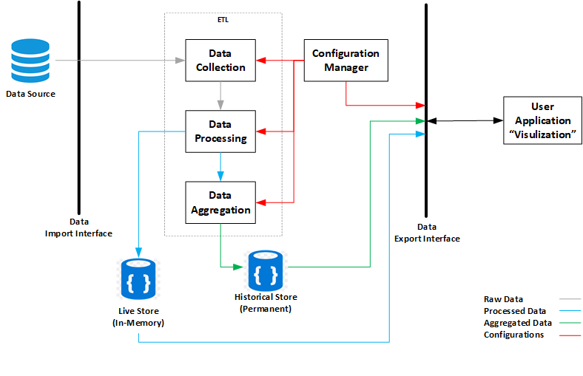
\includegraphics[scale=0.9]{images/architektur_uebersicht.png}
    \caption{Systemarchitektur Uebersicht}
    \label{img:architektur_uebersicht}
\end{figure}
Am Anfang (Links) bei der „Data Source“ (Datenquelle) werden alle Daten aus der MIC Datenbank genommen. Im Kapitel Extract [\ref{sec:extract}] wird noch genauer darauf eingegangen wie der Prozess Abläuft. 
Sobald die Daten extrahiert sind werden sie verarbeitet, Aggregiert (Kapitel Transform [\ref{sec:transform}])  und entweder in die Redis In-Memory Datenbank oder in den Permanenten Speicher der Cassandra Datenbank gespeichert (Kapitel Load [\ref{sec:load}]). 
Schlussendlich kommen die Daten aus den Datenbanken über eine REST [\ref{sec:REST}] Schnittstelle in den Visualisierungsprozess (Kapitel Visualization [\ref{sec:visualization}]). Dort kommen sie in eine Elasticsearch [\ref{sec:ES}] Datenbank, um dem Visualisierungstool Kibana [\ref{ssec:Kibana}] optimalen Zugriff zu verschaffen.
Der „Configuration Manager“ ist in unserer Diplomarbeit leider weggefallen, weil unsere Arbeit nur einen Prototypen darstellen soll und wir uns deswegen auf die wichtigsten Dinge Konzentriert haben.
Folgend werden die Schritte einzeln Erklärt wie sie geplant waren.
\subsection{Import-Interface}
Dieses Modul soll eine Verbindung zu Datenquellen und API's [\ref{sec:API} herstellen um auf der Datenquelle Abfragen ausführen zu können. Datenquellenspezifische Dinge wie, … (hide, network, security and query issues from the system)… sollen abstrahiert werden.
\begin{figure}[H]
    \centering
    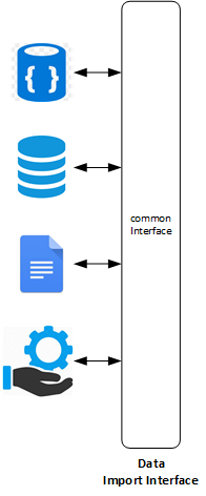
\includegraphics[scale=1]{images/arch_dataImportInterface.png}
    \caption{Systemarchitektur Import-Interface}
    \label{img:arch_dataImportInterface}
\end{figure}
Beim Import soll durch ein Interface eine zusätzliche Schicht auferlegt werden um Daten
in den verschiedensten Formaten entgegennehmen zu können. Dieser modulare Ansatz
ermöglicht es auch durch ein simples Tauschen der Module an eine anderen
Systemschnittstellen sich einzuwählen. 
\subsection{Data-Collection}
Dieses Modul soll periodisch Daten von der Datenquellen ziehen. Abhängig von dem Datenformat müssen wir ggf. die Daten parsen um diese weiterzuverarbeiten. Mit den gelieferten Daten bilden wir dann ein Unified-Object, diesem fügen wir einen Zeitstempel und eine Stream-ID (zur späteren Identifikation) hinzu.
\begin{figure}[H]
    \centering
    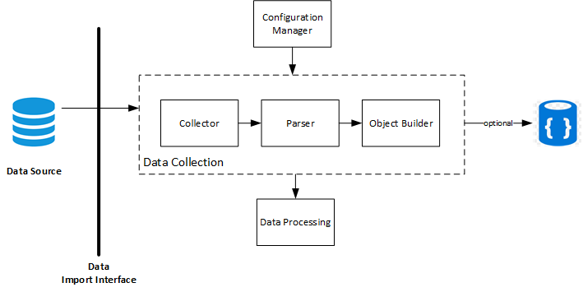
\includegraphics[scale=1]{images/archDataCollection.png}
    \caption{Systemarchitektur Data-Collection}
    \label{img:archDataCollection}
\end{figure}
\subsection{Data-Processing}
Wie folgende Grafik zeigt bekommt das Modul rohe Datenströme aus dem Data-Collection Modul.

Im Modul können verschiedenste Verarbeitungsmethoden angewendet werden. Um zum Beispiel bestimmte Daten herauszufiltern welche nicht benötigt werden. Eine andere Möglichkeit wäre aber auch Datensätze die Gemeinsamkeiten Aufweisen auf einen Gemeinsamen Datensatz zusammenzuführen. Nachdem wir Dokumentenorientierte Datenbanken verwenden ist die Schemafreiheit an dieser Stelle besonders Wichtig. 

Sobald die Prozesse fertig sind kommen die bearbeiteten Datenströme in das nächste Modul die Daten Aggregation. Optional werden die Daten auch in einer In-Memory Datenbank zwischengespeichert.
\begin{figure}[H]
    \centering
    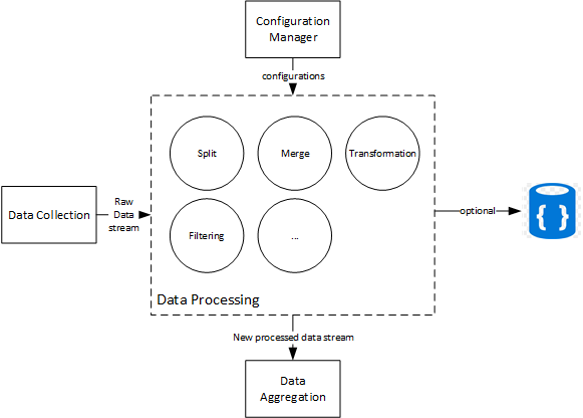
\includegraphics[scale=1]{images/archDataProcessing.png}
    \caption{Systemarchitektur Data-Processing}
    \label{img:archDataProcessing}
\end{figure}
\subsection{Data-Aggregation}
Die verarbeiteten Daten kommen in das Aggregations Modul. Das Aggregations Modul besitzt zwei verschiedene Konfigurationen nämlich den Aggregationsplan und die Aggregationsfunktion. In der Folgenden Grafik wird Dargestellt wie diese Aggregationen aussehen können. Außerdem können mehrere Aggregationspläne für dieselben Daten definiert werden. 

Sobald die Daten Aggregiert wurden kommen sie in den Permanenten Speicher
\begin{figure}[H]
    \centering
    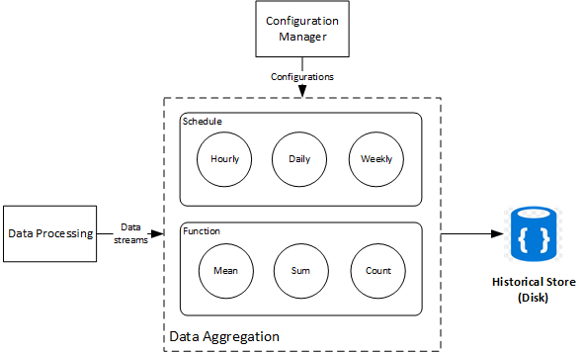
\includegraphics[scale=1]{images/archDataAggregation.png}
    \caption{Systemarchitektur Data-Aggregation}
    \label{img:archDataAggregation}
\end{figure}
\subsection{Data-Interface}
Das Dateninterface ist die Zentrale Schnittstelle um die zuvor verarbeiteten Daten in die Visualisierungsapplikation zu bekommen.
Dieses Interface wird als REST [\ref{sec:REST} Schnittstelle realisiert. Somit kann auf den Permanenten Speicher sowie als auch auf die Live Daten Abfragen gemacht werden. Die Visualisierungsapplikation kann auch eine Metabeschreibung der Daten (Namen, Typen usw.) abrufen.
\begin{figure}[H]
    \centering
    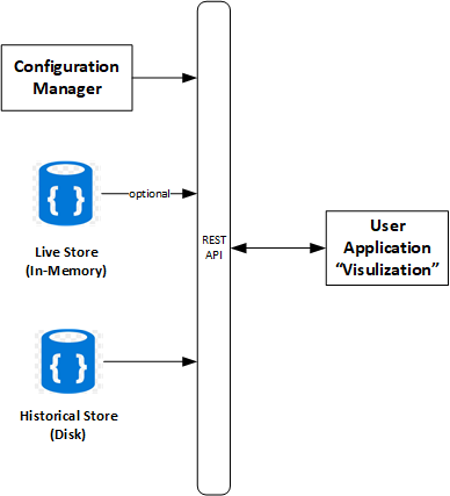
\includegraphics[scale=1]{images/archDataInterface.png}
    \caption{Systemarchitektur Data-Interface}
    \label{img:archDataInterface}
\end{figure}